\section{Negative Selection Algorithm}

\begin{frame}
\begin{center}
\begin{spacing}{2.0}
 \Huge {Negative Selection Algorithm}
 \large {\\Li, Meizhen}
\end{spacing}
\end{center}
\end{frame}


\begin{frame}{Inspiration-Biological immune system}
  \begin{itemize}
  \item {
    The antigen-antibody reaction is an exclusive process.
  }
  \item {
    The primary role of immune system is to distinguish self from non-self.
  }
  \item {
    Immune cells are tolerant to self antigens but activate defense mechanisms when recognize non-self antigens.   
  }
  \item {
    The negative selection of T cells happened in the thymus during maturation.
  }
  \end{itemize}
\end{frame}

\begin{frame}{Biological immune system}
  \begin{figure}[hb]
  \centering
  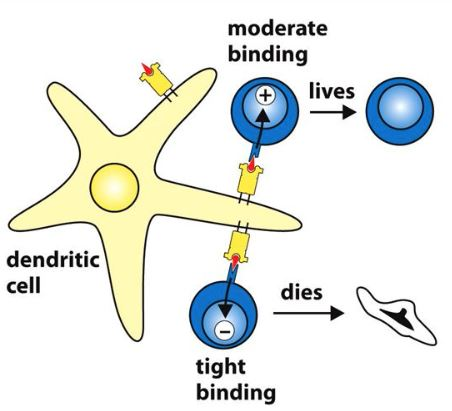
\includegraphics[width=0.6\textwidth]{img/NST.JPG}
  \caption{Negative selection of T cells}
  \end{figure}
\end{frame}

\begin{frame}{Biological immune system}
  \begin{figure}[hb]
  \centering
  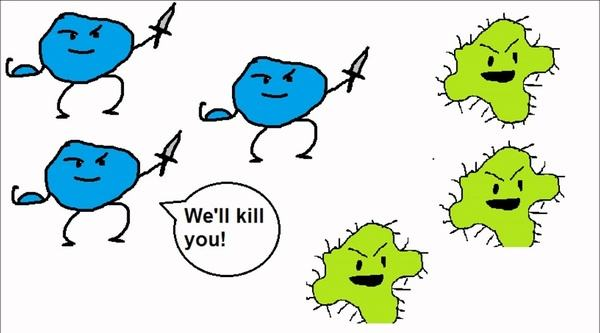
\includegraphics[width=0.6\textwidth]{img/ag_ab.jpg}
  \caption{Antigen-antibody interaction}
  \end{figure}
\end{frame}

% You can reveal the parts of a slide one at a time
% with the \pause command:
\begin{frame}{Defining the NSA}
  \begin{itemize}
  \item<1->{
    Define Self as a normal pattern of activity or stable behavior of a system/process.\\
    -Represent the collection as multiset of S of strings of length \emph{l} over a finite alphabet.
  }
  \item<2-> {   
    Generate a set R of detectors,each of which fails to match any string in S.
  }
  % You can also specify when the content should appear
  % by using <n->:
  \end{itemize}
\end{frame}
 
\begin{frame}{Flowchart}
  \begin{figure}[hb]
  \centering
  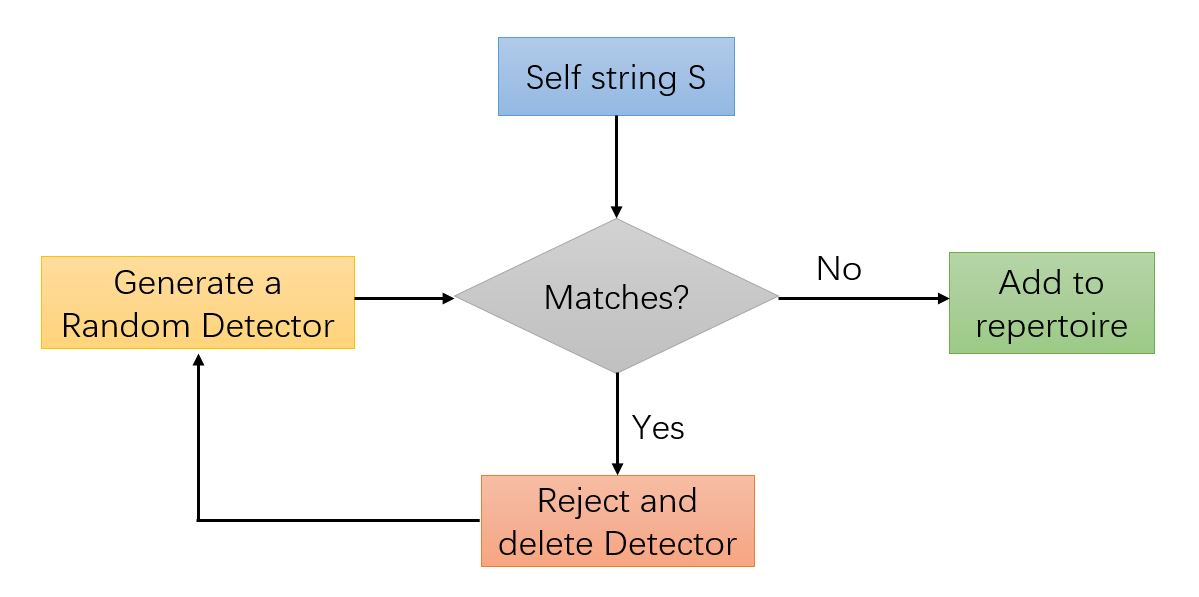
\includegraphics[width=0.8\textwidth]{img/NSAflowchart1.jpg}
  \caption{Generation of effective detector}
  \end{figure}
\end{frame}

\begin{frame}{Pseudocode}
 \begin{algorithm}[H]
  \caption{Detector Generation}          
  \label{alg1}      % and a label for \ref{} commands later in the document
    \begin{algorithmic}  
       \STATE Input:SelfData
       \STATE Output:Repertoire
       \STATE Repertoire $\Leftarrow$ emptyset
       \WHILE {$ !StopCondition()$}
       \STATE Detectors $\Leftarrow$ GenerateRandomDetectors()
       \FOR {Detector[i] $\in$ Repertoire }
       \IF {$not$ Matches(Detector[i],SelfData)}
       \STATE Repertoire $\Leftarrow$ Detector[i]
       \ENDIF
       \ENDFOR
       \ENDWHILE
       \STATE Return (Repertiore)

    \end{algorithmic}
  \end{algorithm} 
\end{frame}

\begin{frame}{Defining the NSA}
  \begin{itemize}
  \item {
    Monitor new observations for changes by continually testing the detectors matching against representatives of S.  If any detector ever matches, a change must have occurred in system behavior.
  }
  \end{itemize}
\end{frame}

\begin{frame}{Flowchart}
  \begin{figure}[hb]
  \centering
  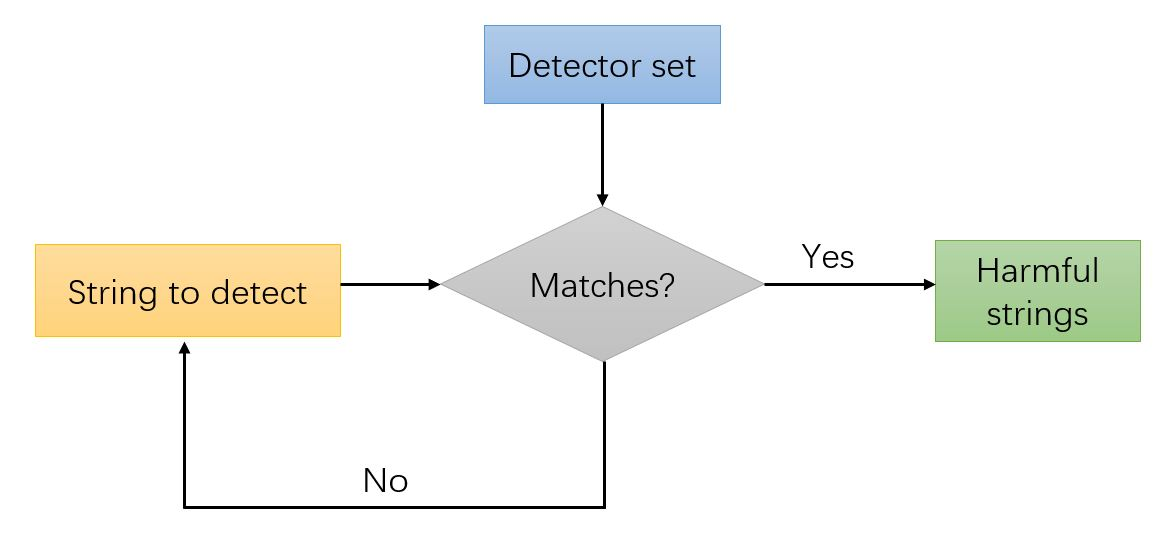
\includegraphics[width=0.8\textwidth]{img/NSAflowchart2.jpg}
  \caption{Detector application}
  \end{figure}
\end{frame}

\begin{frame}{Pseudocode}
 \begin{algorithm}[H]
  \caption{Detector Monitering}          
  \label{alg2}      
    \begin{algorithmic}  
       \STATE Input:InputSamples,Repertoire
  
       \FOR {Input[i] $\in$ InputSamples}
       \STATE Inputiclass $\Leftarrow$ nonself  
       \FOR {Detector[j] $\in$ Repertoire }
       \IF {Matches(Detector[j],SelfData)}
       \STATE Inputiclass $\Leftarrow$ self
       \ENDIF
       \ENDFOR
       \ENDFOR            
    \end{algorithmic}
  \end{algorithm} 
\end{frame}
